\chapter{Source detection: denoising and background modeling}
\label{ch_background}

% \markright{Source detection: denoising and background modeling}

\section{Method}
In some cases such as for Fermi data, the diffuse emission from the Milky Way  makes a relatively intense background. We have to extract this background in order to detect point sources. This diffuse interstellar emission may be modeled, and we want to use such a background model and incorporate a background removal in our denoising algorithm.

We note $\mathbf{Y}$ the data, $\mathbf{B}$ the background we want to remove, and $d^{(b)}_{j}[k]$ the MS-VSTS coefficients of $\mathbf{B}$ at scale $j$ and position $k$. We determine the multi-resolution support by comparing $|d_j[k]-d^{(b)}_{j}[k]|$ with $\kappa \sigma_j$.

We formulate the reconstruction problem as a convex constrained minimization problem:

\begin{equation}
\label{bgr_eq34}
\begin{split}
\text{Arg} \min_{\mathbf{X}} \| \mathbf{ \Phi}^{T}\mathbf{X}\|_1,
\text{s.t.} \\ \: \left\{\begin{array}{c}\mathbf{X} \geqslant 0 , \\\forall (j,k)\in \mathcal{M},      (\mathbf{ \Phi}^{T}\mathbf{X})_j[k]=(\mathbf{ \Phi}^{T}(\mathbf{Y} - \mathbf{B}))_j[k] , \end{array}\right.
\end{split}
\end{equation}

Then, the reconstruction algorithm scheme becomes:
\begin{eqnarray}
\tilde{\mathbf{X}} = P_{+}[\mathbf{ X}^{(n)} + \mathbf{ \Phi} P_{\mathcal{M}} \mathbf{ \Phi}^{T} (\mathbf{ Y} - \mathbf{B} - \mathbf{ X}^{(n)})] , \\
\mathbf{X}^{(n+1)} = \mathbf{ \Phi}\text{ST}_{\lambda_n}[\mathbf{ \Phi}^{T}\tilde{\mathbf{X}}].
\end{eqnarray}

\begin{figure}[htb]
\begin{center}
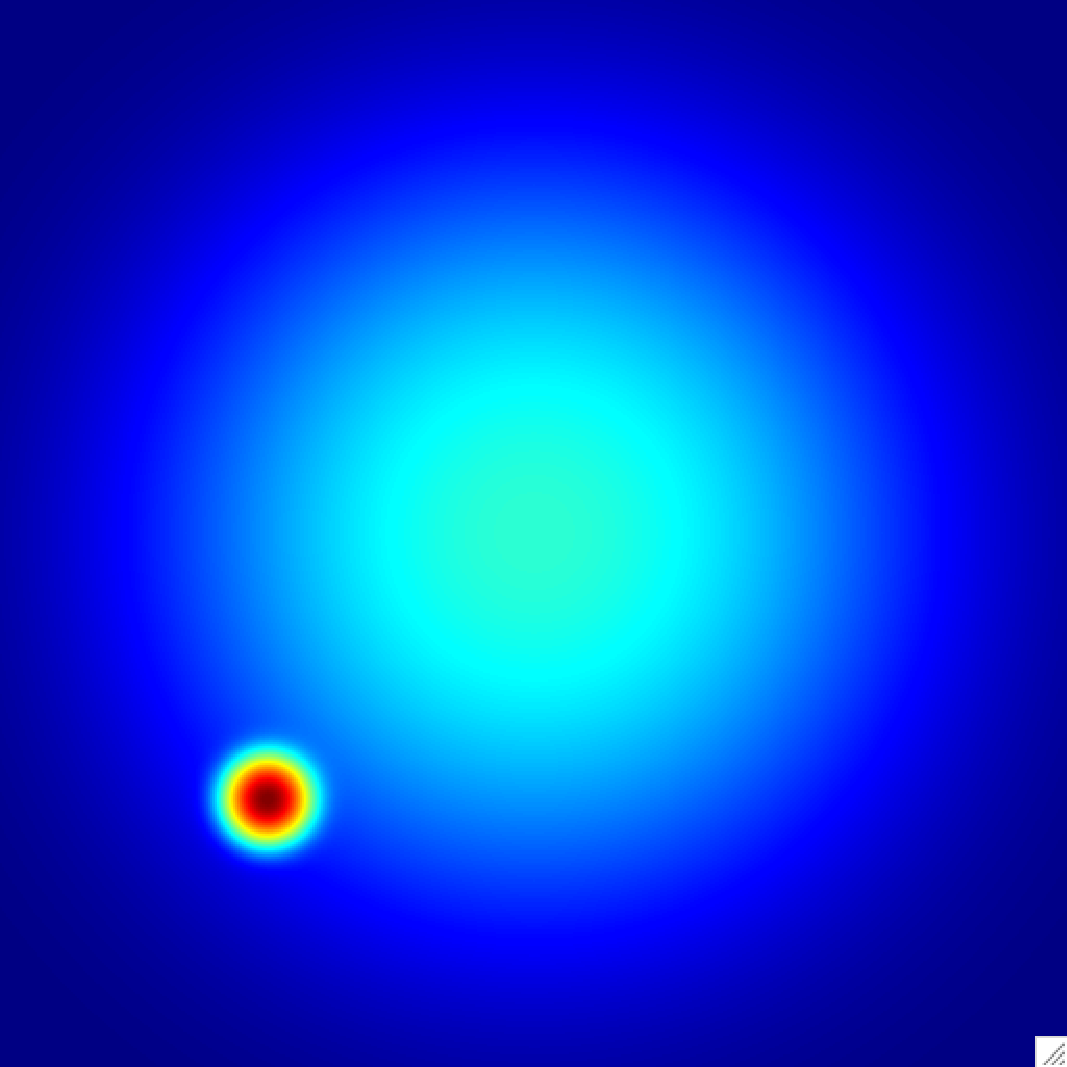
\includegraphics[width=2.9in]{13822fg24.pdf} \hfill
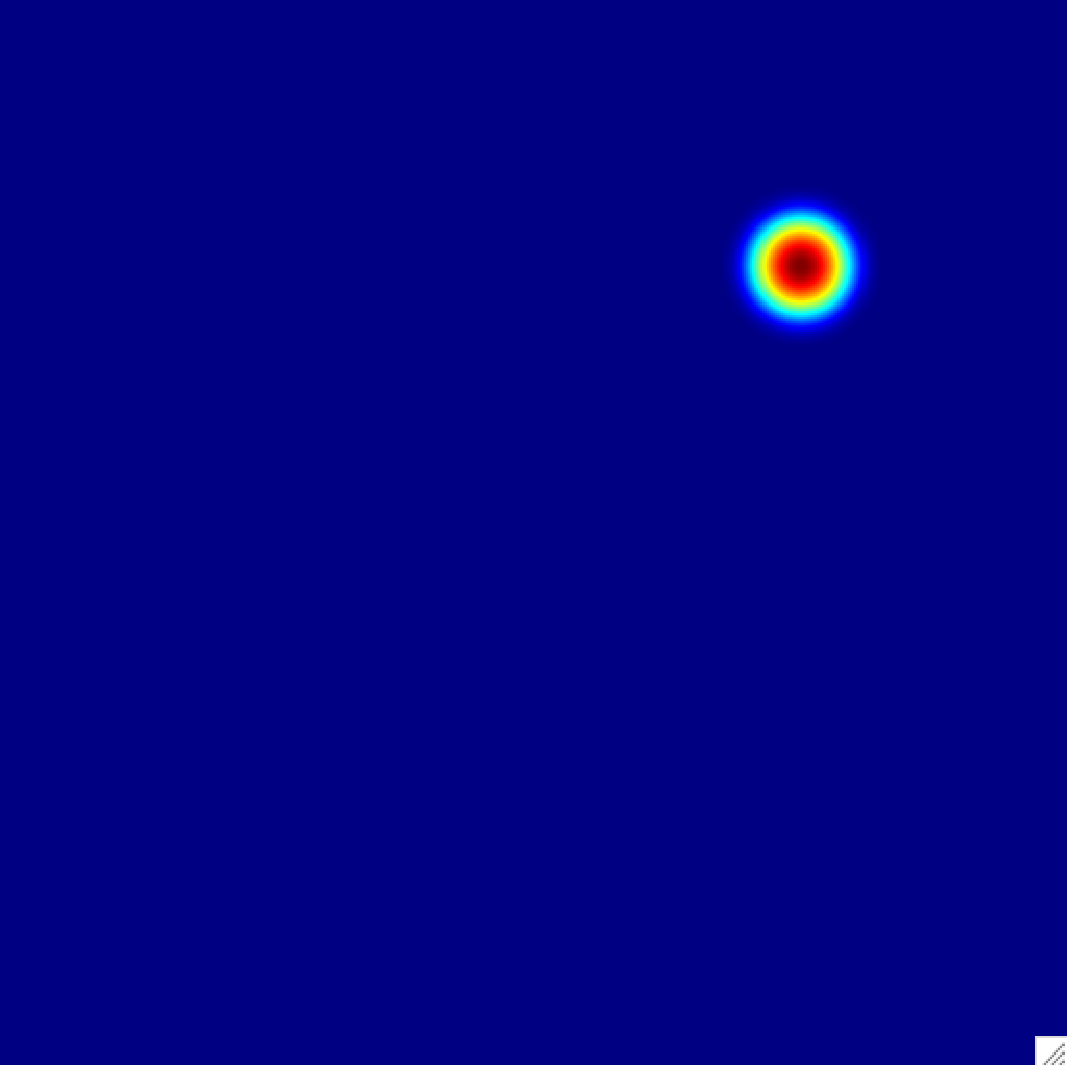
\includegraphics[width=2.9in]{13822fg25.pdf} \hfill
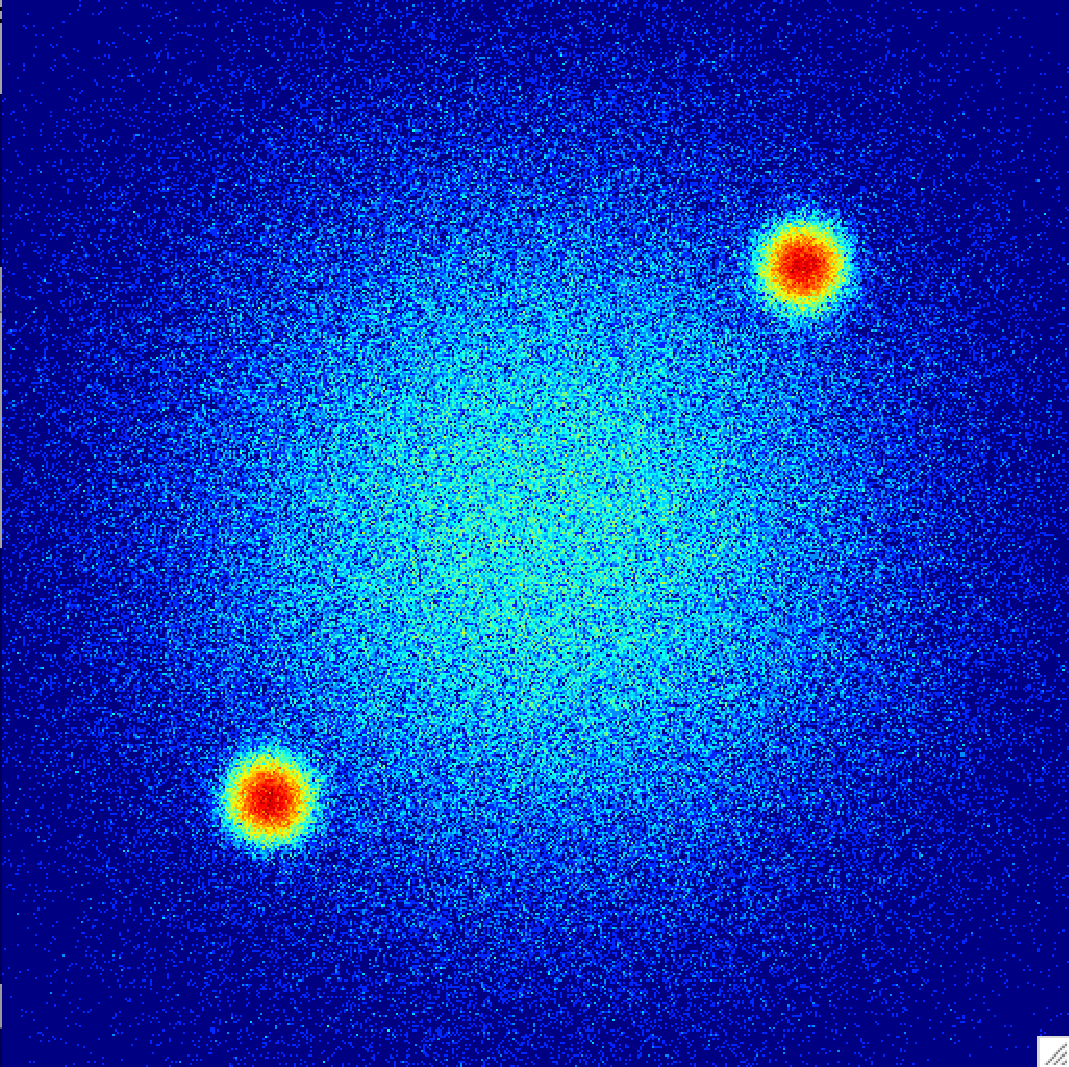
\includegraphics[width=2.9in]{13822fg26.pdf} \hfill
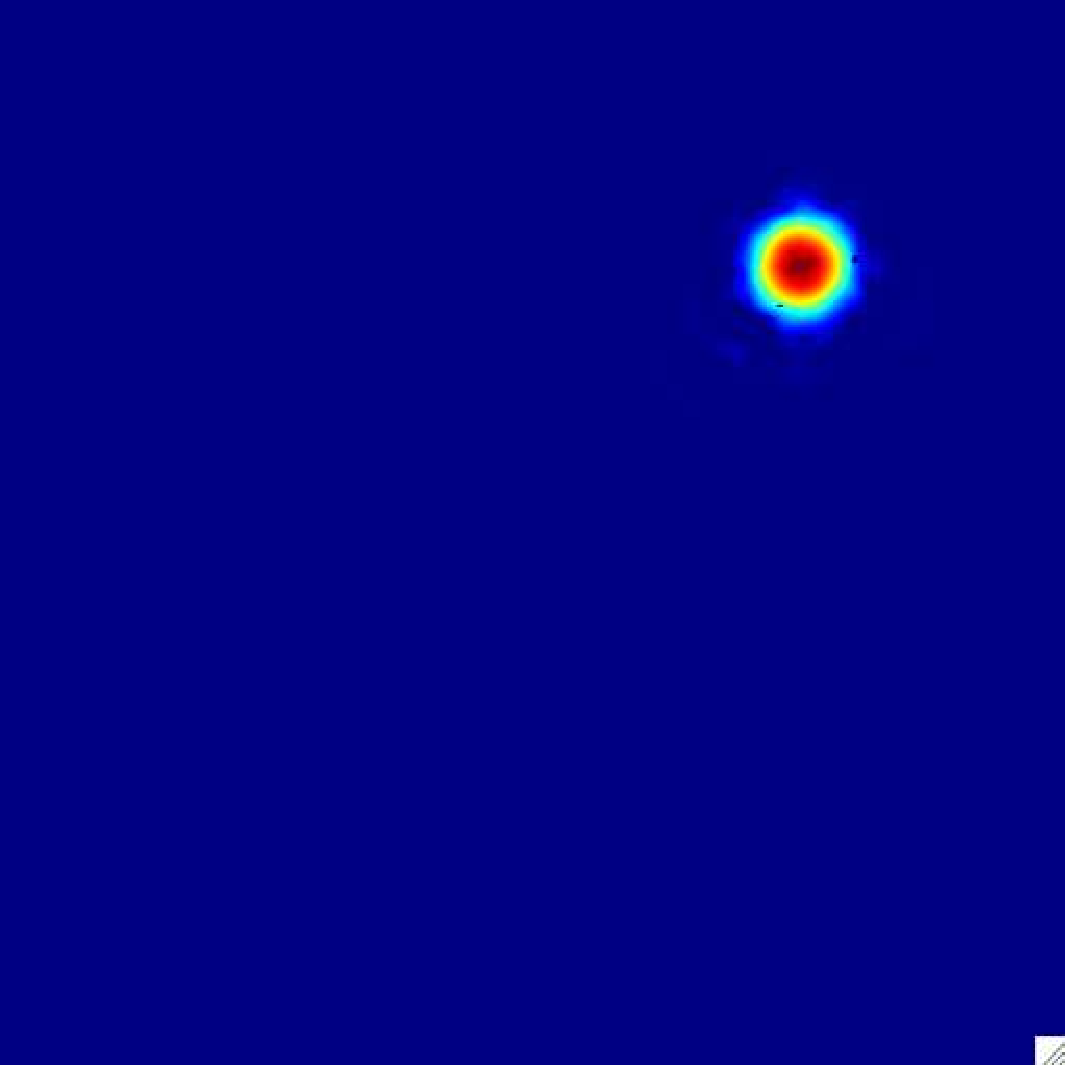
\includegraphics[width=2.9in]{13822fg27.pdf}
\caption{Theoretical testing for MS-VSTS + IUWT denoising + background removal algorithm (Algorithm~\ref{alg3}). View on a single HEALPix face.
\emph{Top Left}: Simulated background : sum of two Gaussians of standard deviation equal to 0.1 and 0.01 respectively.
\emph{Top Right}: Simulated source: Gaussian of standard deviation equal to 0.01.
\emph{Bottom Left}: Simulated poisson data.
\emph{Bottom Right}: Image denoised with MS-VSTS + IUWT and background removal.
}
\label{background}
\end{center}
\end{figure}
The algorithm is illustrated by the theoretical study in Figure~\ref{background}. We denoise Poisson data while separating a single source, which is a Gaussian of standard deviation equal to 0.01, from a background, which is a sum of two Gaussians of standard deviation equal to 0.1 and 0.01 respectively. 

\begin{algorithm}
\caption{MS-VSTS + IUWT Denoising + Background extraction}
\label{alg3}

\begin{algorithmic}[1]
\REQUIRE $\quad$ data $a_0:=\mathbf{Y}$, background $B$, number of iterations $N_{\max}$, threshold $\kappa$. \\
\underline{\emph{\textbf{Detection}}} \\
\FOR{$j=1$ to $J$}
\STATE Compute $a_j$ and $d_j$ using (\ref{eq27}).
\STATE Hard threshold $(d_j[k] - d^{(b)}_{j}[k])$ with threshold $\kappa \sigma_j$ and update $\mathcal{M}$.
\ENDFOR \\
\underline{\emph{\textbf{Estimation}}} \\
\STATE Initialize $\mathbf{X}^{(0)}=0$, $\lambda_0 = 1$.
\FOR{$n=0$ to $N_{\max}-1$}
\STATE $\tilde{\mathbf{X}}= P_{+}[\mathbf{ X}^{(n)} + \mathbf{ \Phi} P_{\mathcal{M}} \mathbf{ \Phi}^{T} (\mathbf{ Y} - \mathbf{B} - \mathbf{ X}^{(n)})]$.
\STATE $\mathbf{X}^{(n+1)} = \mathbf{ \Phi}\text{ST}_{\lambda_n}[\mathbf{ \Phi}^{T}\tilde{\mathbf{X}}]$.
\STATE $\lambda_{n+1} = \frac{N_{\max} - (n+1)}{N_{\max} - 1}$.
\ENDFOR
\STATE Get the estimate $\hat{\mathbf{\Lambda}} = \mathbf{X}^{(N_{\max})}$.
\end{algorithmic}
\end{algorithm}

Like Algorithm~\ref{alg1}, Algorithm~\ref{alg3} can be adapted to make multiresolution support adaptation.


\section{Experiment}

We applied Algorithms~\ref{alg3} on simulated Fermi data. To test the efficiency of our method, we detect the sources with the SExtractor routine~\citep{astro:bertin96}, and compare the detected sources with the theoretical sources catalog to get the number of true and false detections. Results are shown on Figures~\ref{sources} and~\ref{sourcesreest}. The SExtractor method was applied on the first wavelet scale of the reconstructed map, with a detection threshold equal to 1. It has been chosen to optimise the number of true detections. SExtractor makes $593$ true detections and $71$ false detections on the Fermi simulated map restored with Algorithm~\ref{alg4} among the $1000$ sources of the simulation. On noisy data, many fluctuations due to Poisson noise are detected as sources by SExtractor, which leads to a big number of false detections (more than 2000 in the case of Fermi data). 

\begin{figure}[htb]
\begin{center}
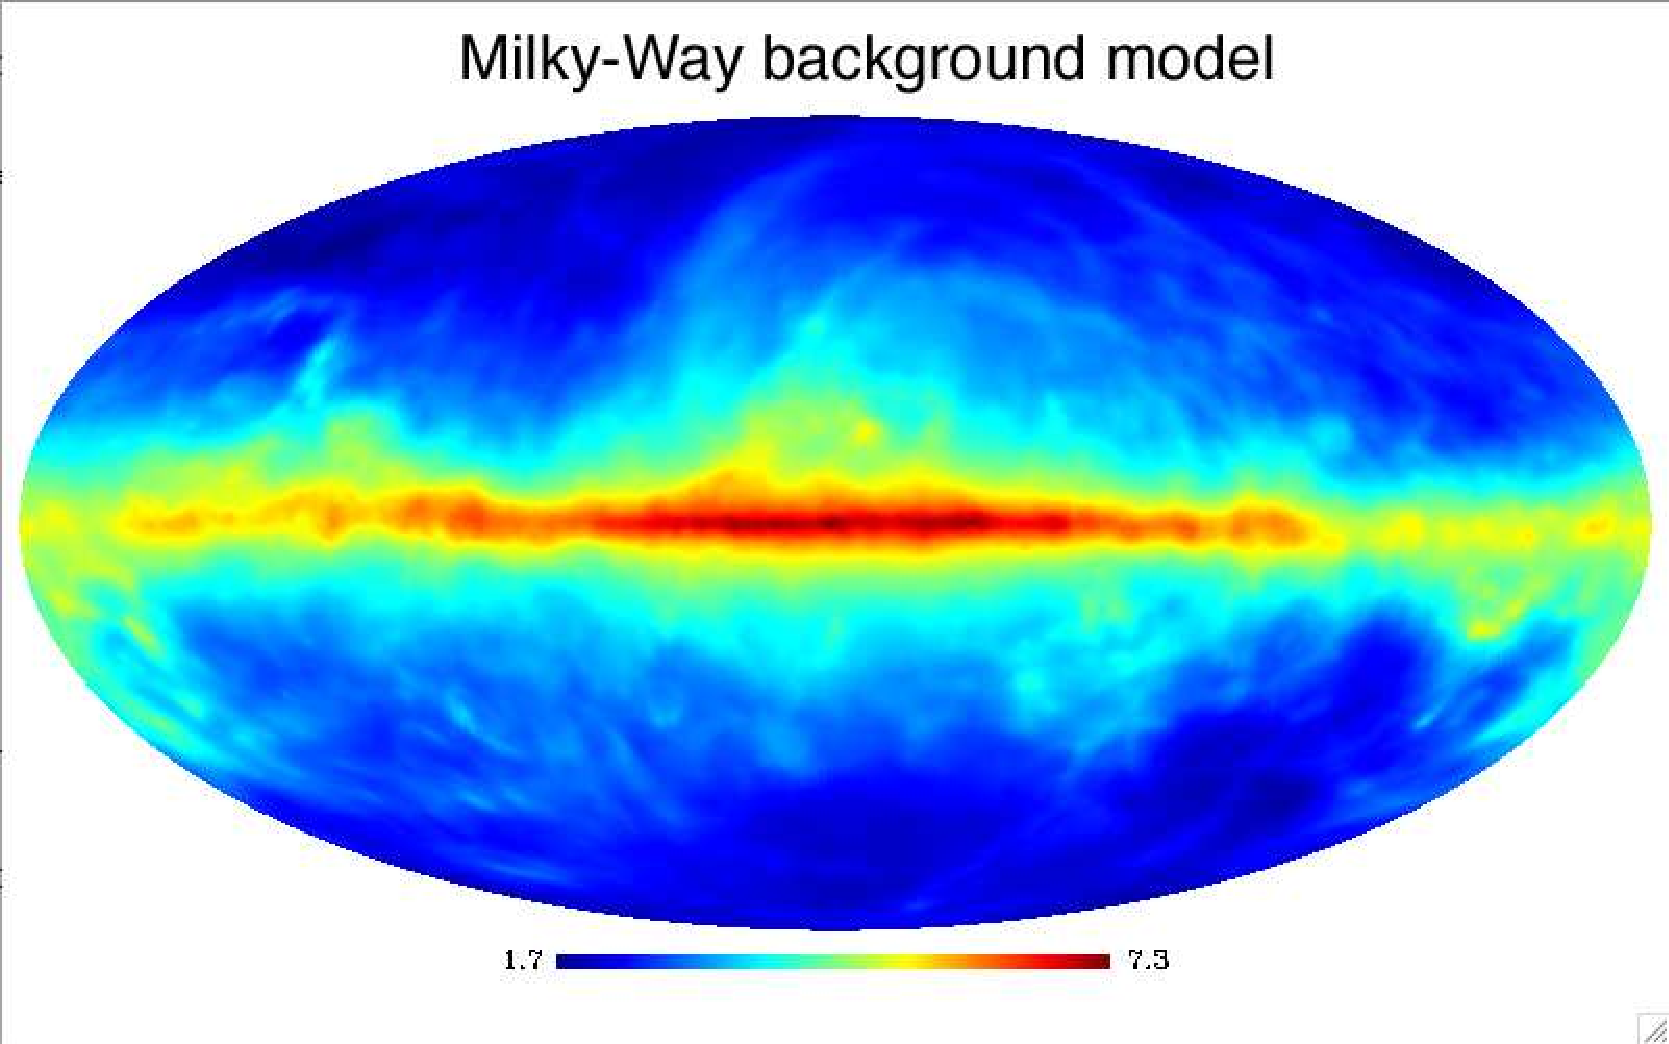
\includegraphics[width=2.9in]{13822fg28.pdf} \hfill
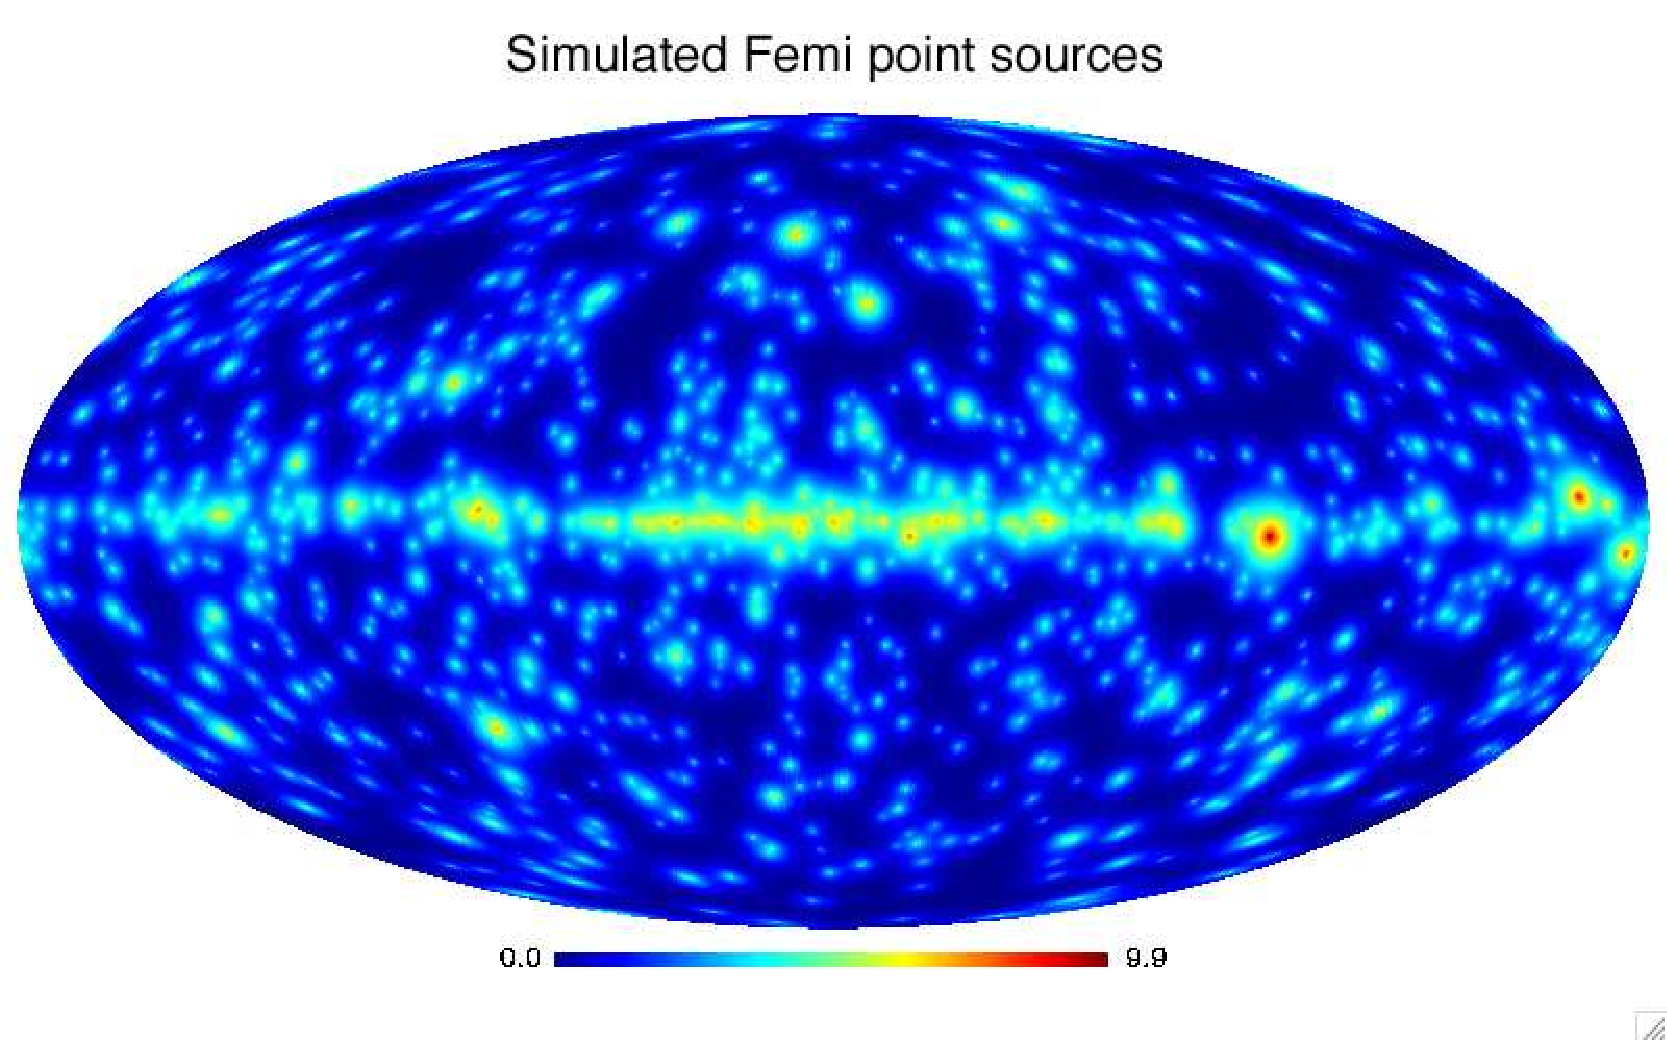
\includegraphics[width=2.9in]{13822fg29.pdf} \hfill
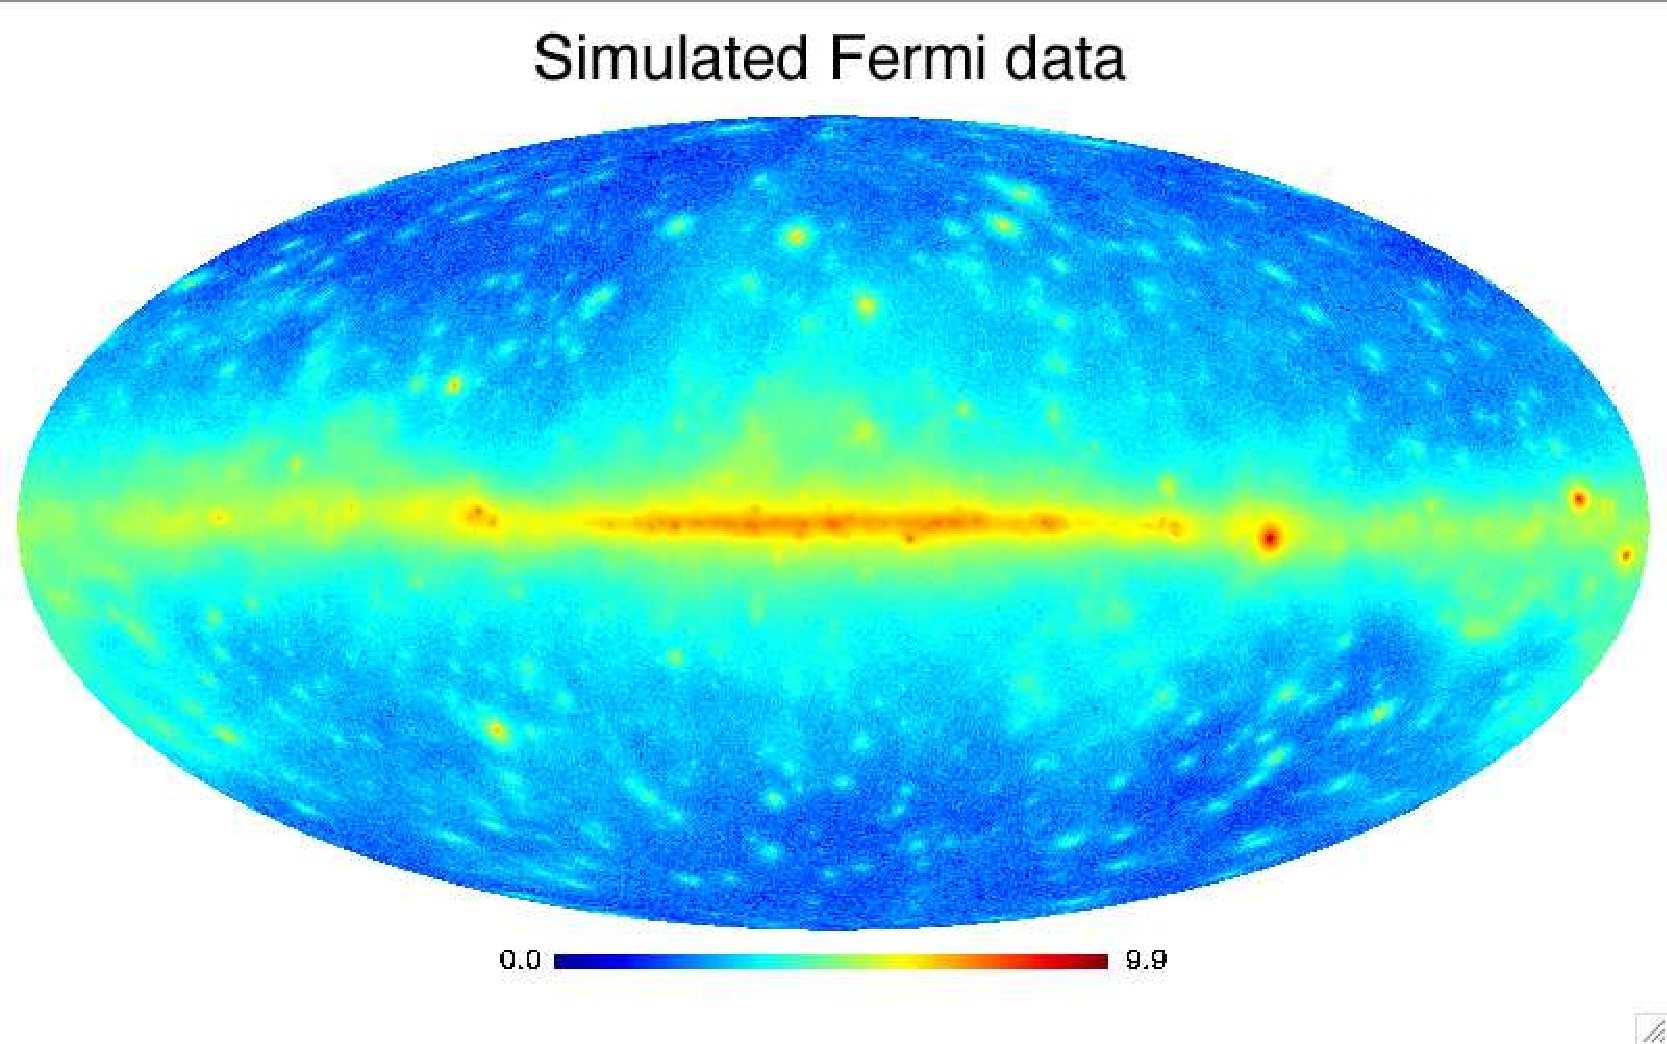
\includegraphics[width=2.9in]{13822fg30.pdf} \hfill
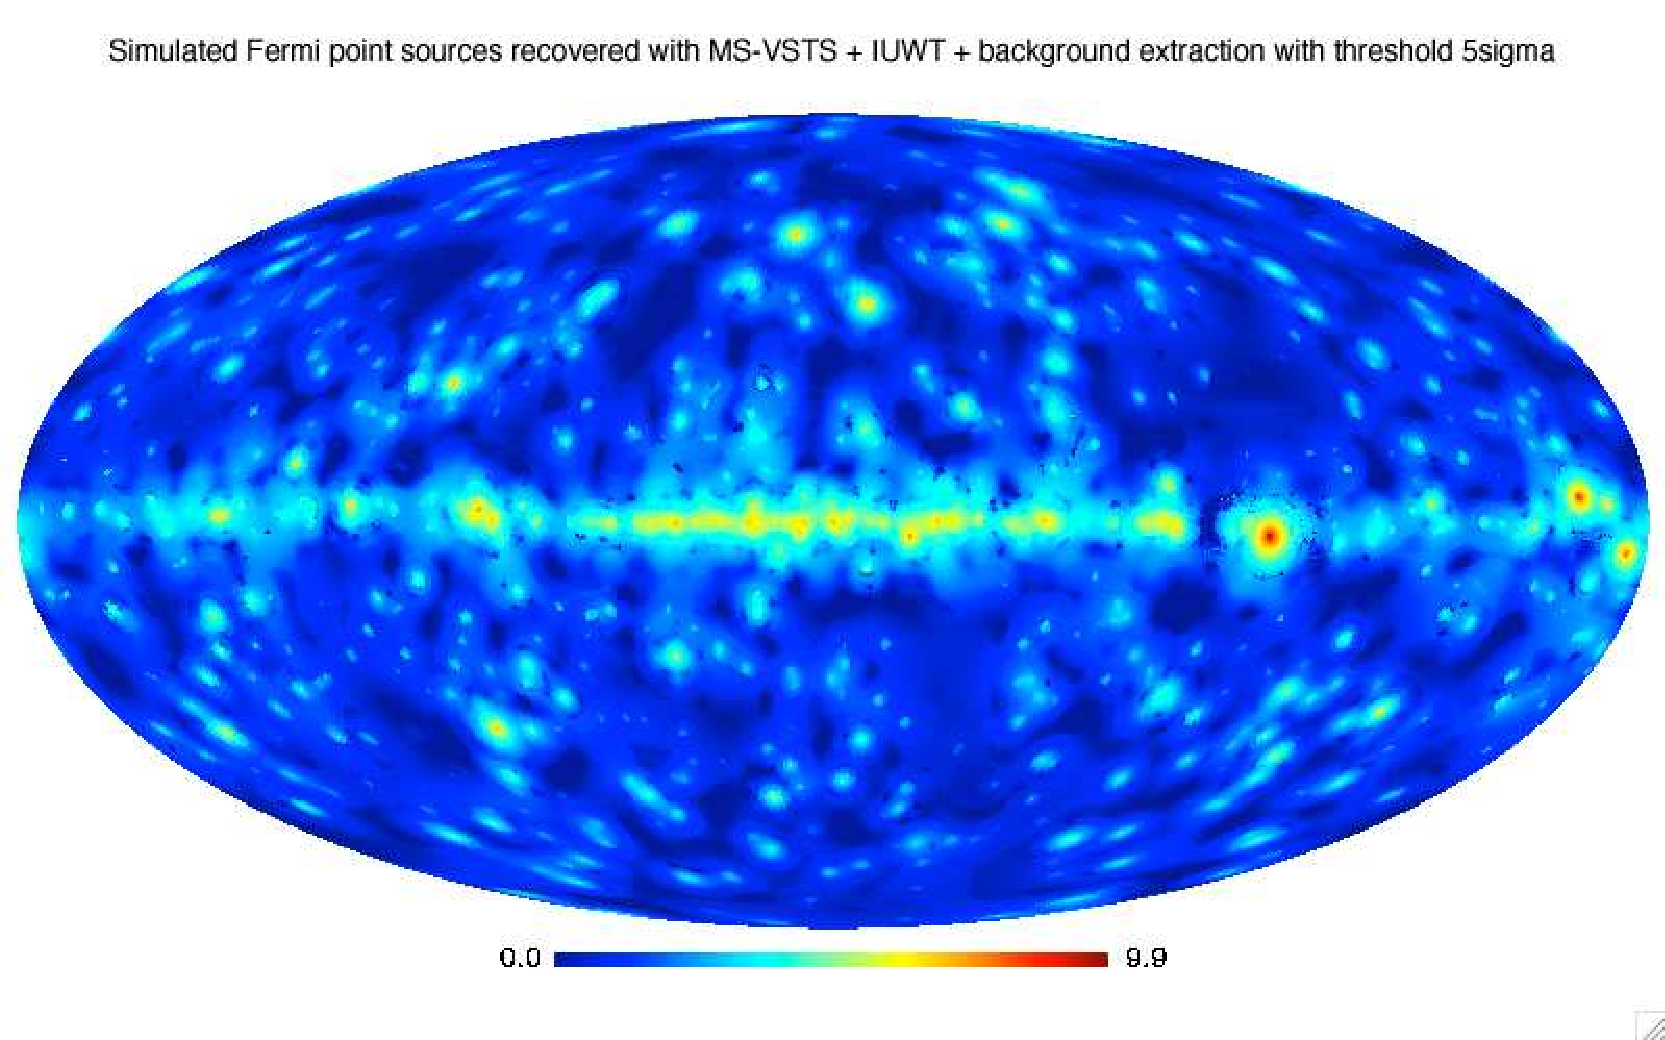
\includegraphics[width=2.9in]{13822fg31.pdf} \hfill
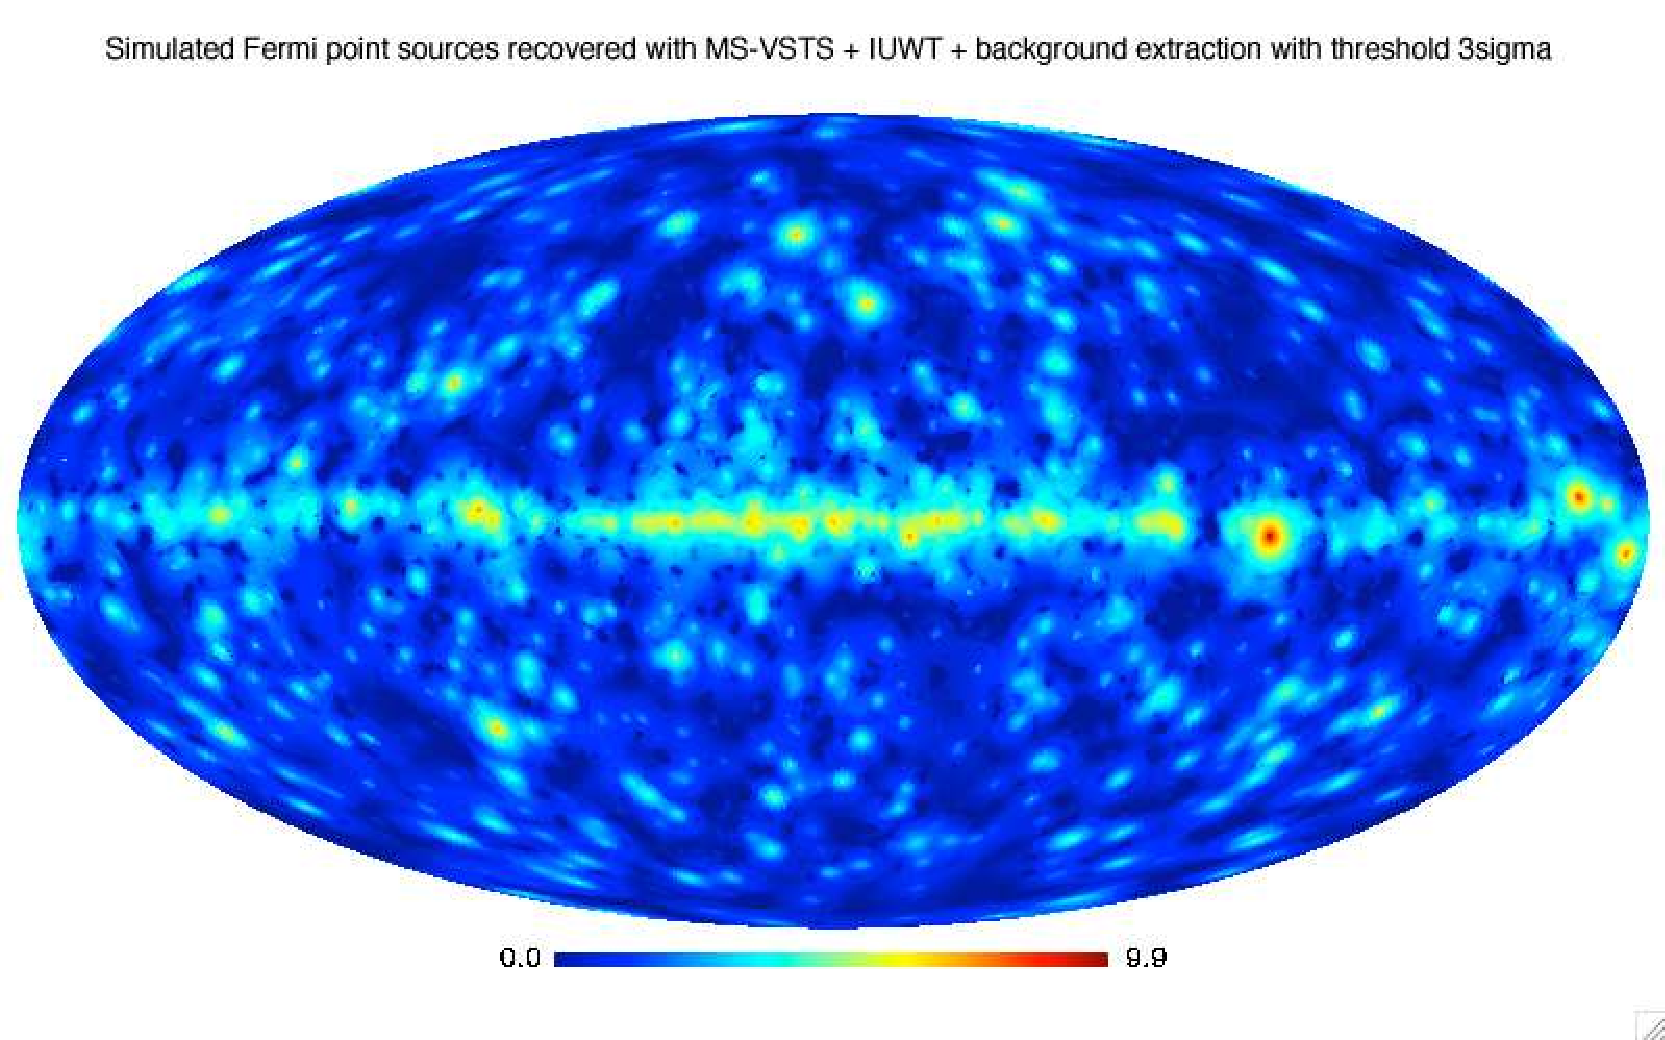
\includegraphics[width=2.9in]{13822fg32.pdf}
\caption{\emph{Top Left}: Simulated background model.
\emph{Top Right}: Simulated Gamma Ray sources.
\emph{Middle Left}: Simulated Fermi data with Poisson noise.
\emph{Middle Right}: Reconstructed Gamma Ray Sources with MS-VSTS + IUWT + background removal (Algorithm~\ref{alg3}) with threshold $5\sigma_j$.
\emph{Bottom}: Reconstructed Gamma Ray Sources with MS-VSTS + IUWT + background removal (Algorithm~\ref{alg3}) with threshold $3\sigma_j$.
Pictures are in logarithmic scale.}
\label{sources}
\end{center}
\end{figure}

\begin{figure}[htb]
\begin{center}
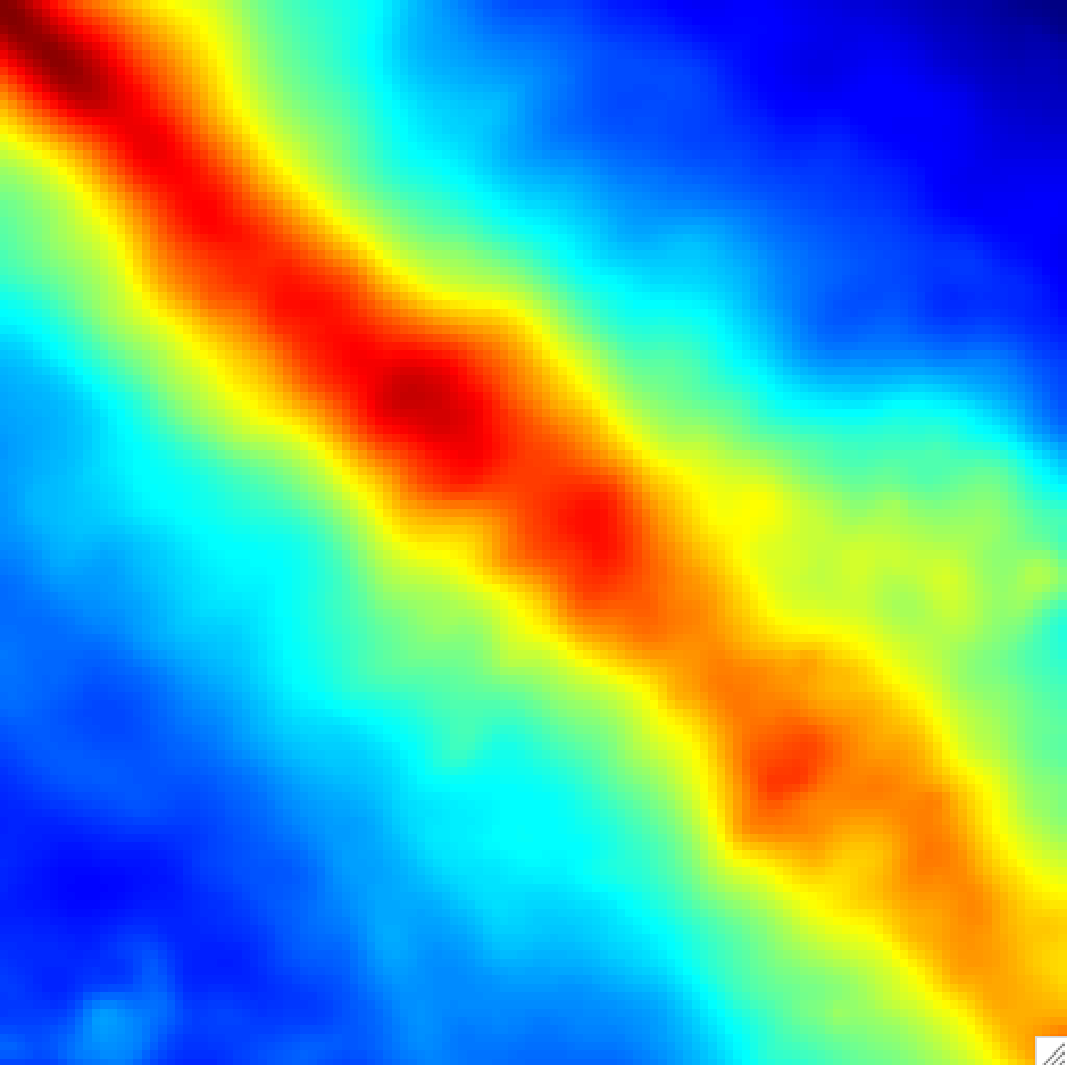
\includegraphics[width=2.5in]{13822fg33.pdf} \hfill
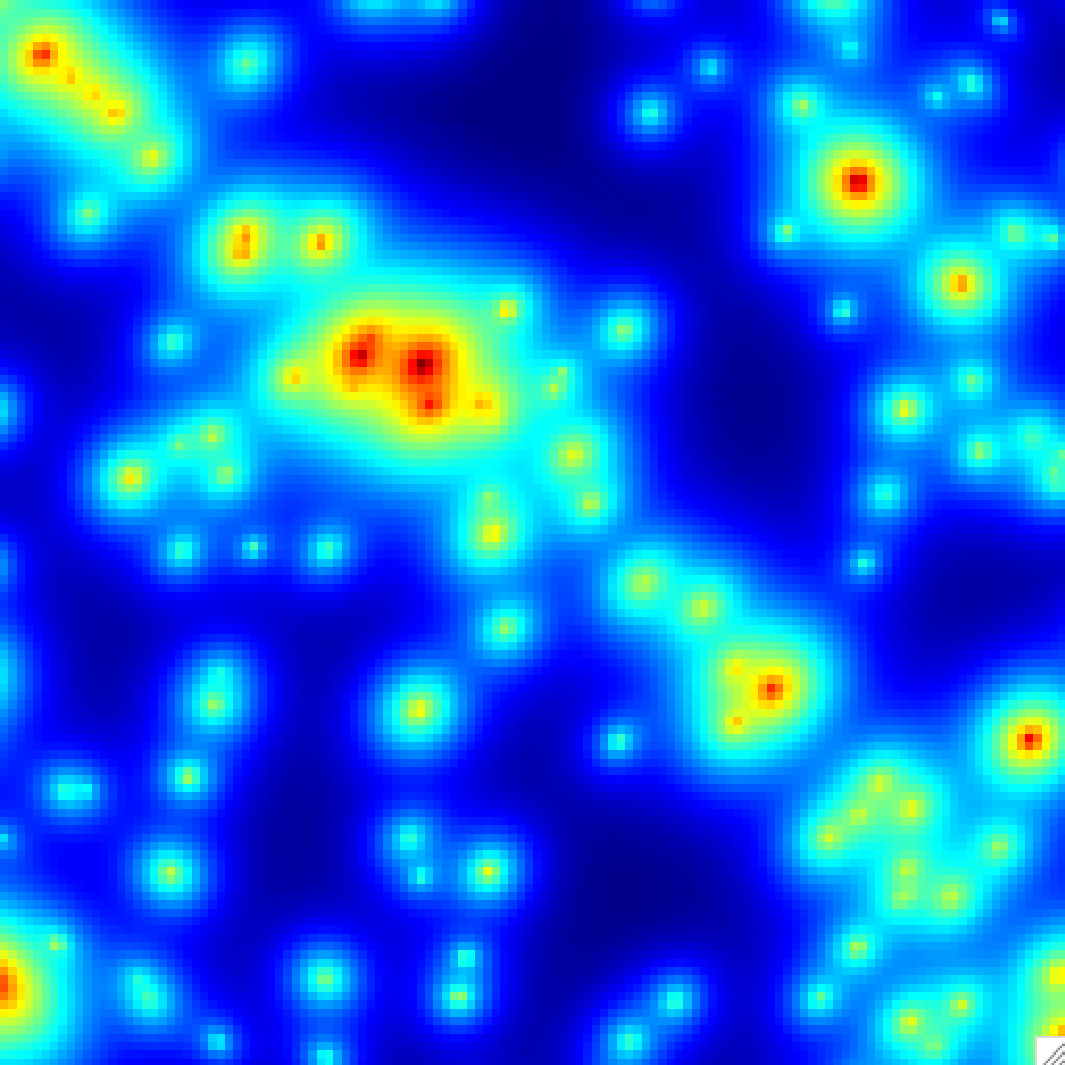
\includegraphics[width=2.5in]{13822fg34.pdf} \hfill
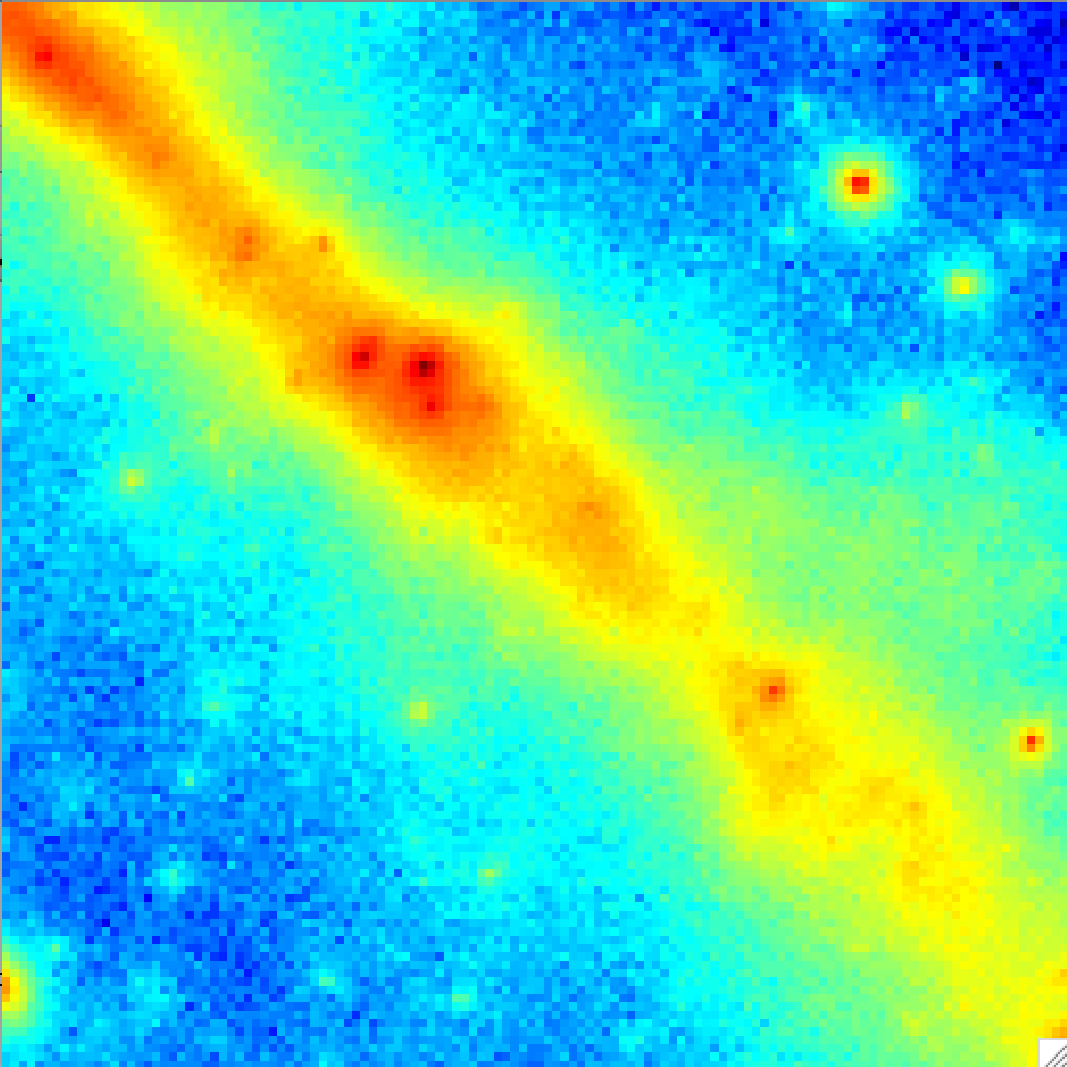
\includegraphics[width=2.5in]{13822fg35.pdf} \hfill
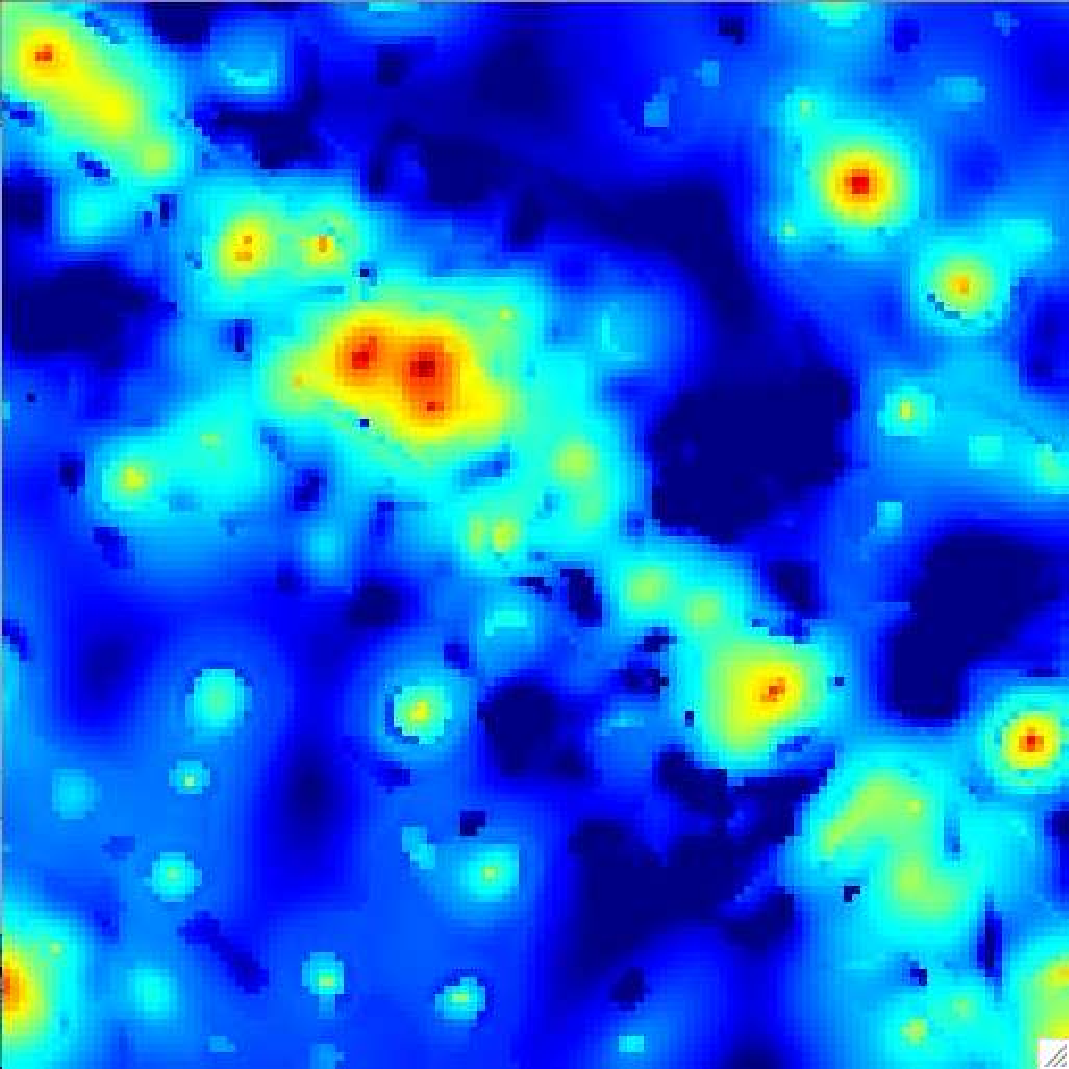
\includegraphics[width=2.5in]{13822fg36.pdf} \hfill
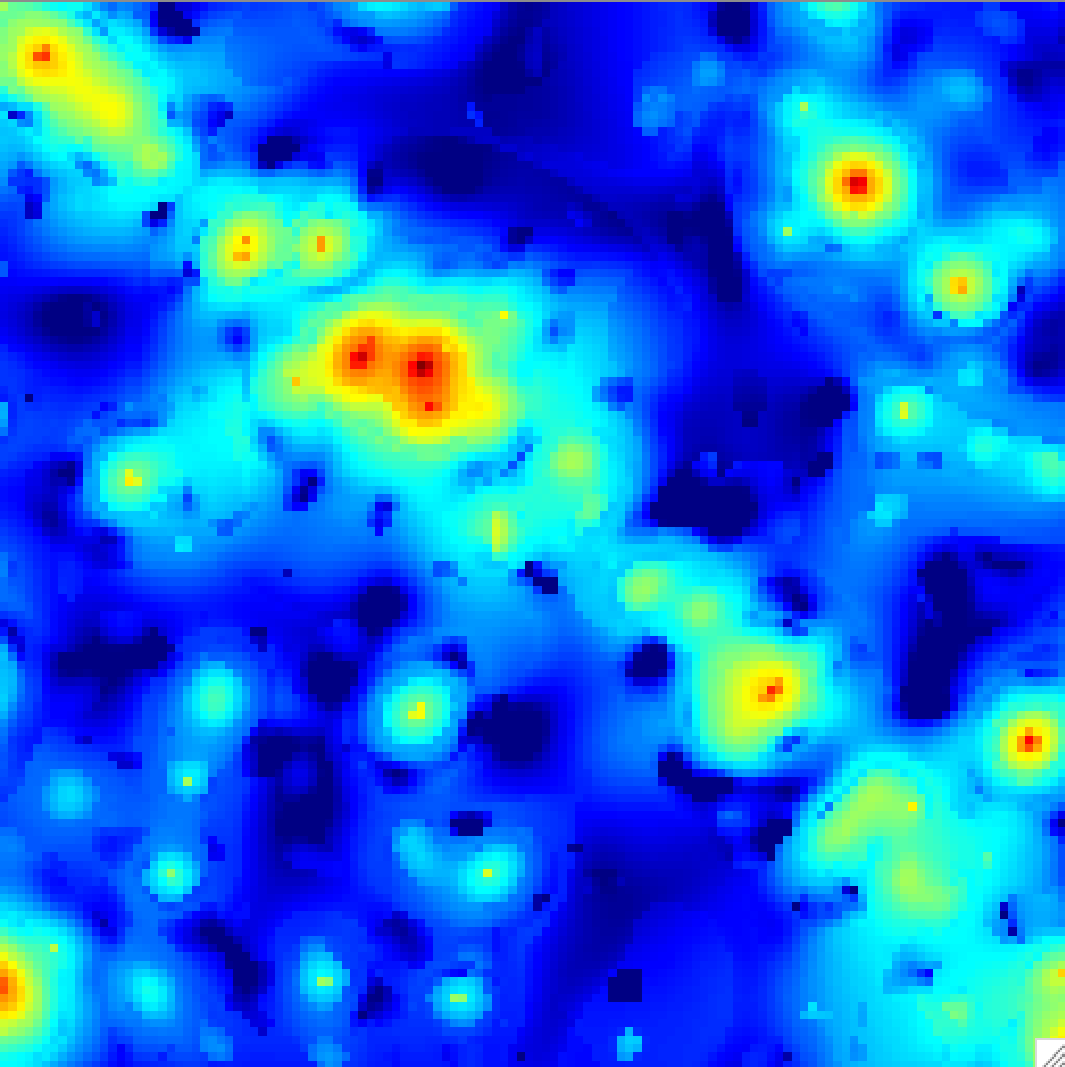
\includegraphics[width=2.5in]{13822fg37.pdf}
\caption{View of a single HEALPix face from the results of Figure~\ref{sources}.\emph{Top Left}: Simulated background model.
\emph{Top Right}: Simulated Gamma Ray sources.
\emph{Middle Left}: Simulated Fermi data with Poisson noise.
\emph{Middle Right}: Reconstructed Gamma Ray Sources with MS-VSTS + IUWT + background removal (Algorithm~\ref{alg3}) with threshold $5\sigma_j$.
\emph{Bottom}: Reconstructed Gamma Ray Sources with MS-VSTS + IUWT + background removal (Algorithm~\ref{alg3}) with threshold $3\sigma_j$.
Pictures are in logarithmic scale.
}
\label{sourcesreest}
\end{center}
\end{figure}



\subsection{Sensitivity to model errors}
\begin{table}
  \centering
  \caption{Percent of true and false detection and signal-noise ratio versus the standard deviation of the Gaussian noise on the background model. 
  }
  \begin{tabular}{|c|c|c|c|}
\hline
Model error std dev & $\%$ of true detect & $\%$ of false detect & SNR (dB) \\
\hline
  0 & $59.3\%$ & $7.1\%$ & 23.8 \\
  10 & $57.0\%$ & $11.0\%$ & 23.2 \\
  20 & $53.2\%$ & $18.9\%$ & 22.6 \\
  30 & $49.1\%$ & $43.5\%$ & 21.7 \\
  40 & $42.3\%$ & $44.3\%$ & 21.0 \\
  50 & $34.9\%$ & $39.0\%$ & 20.3 \\
  60 & $30.3\%$ & $37.5\%$ & 19.5 \\
  70 & $25.0\%$ & $34.6\%$ & 18.9 \\
  80 & $23.0\%$ & $28.5\%$ & 18.7 \\
  90 & $23.6\%$ & $27.1\%$ & 18.3 \\  
\hline
\end{tabular}
  
  \label{table1}
\end{table}

As it is difficult to model the background precisely, it is important to study the sensitivity of the method to model errors. We add a stationary Gaussian noise to the background model, we compute the MS-VSTS + IUWT with threshold $3\sigma_j$ on the simulated Fermi Poisson data with extraction of the noisy background, and we study the percent of true and false detections with respect to the total number of sources of the simulation and the signal-noise ratio ($\text{SNR} (dB) = 20 \log (\sigma_{signal} / \sigma_{noise})$) versus the standard deviation of the Gaussian perturbation. Table~\ref{table1} shows that, when the standard deviation of the noise on the background model becomes of the same range as the mean of the Poisson intensity distribution ($\lambda_{\text{mean}} = 68.764$), the number of false detections increases, the number of true detections decreases and the signal noise ratio decreases. While the perturbation is not too strong (standard deviation $< 10$), the effect of the model error remains low.

